% Created 2024-12-09 Mon 19:32
% Intended LaTeX compiler: pdflatex
\documentclass[10pt,table,dvipsnames,compress]{beamer}
\usepackage[utf8]{inputenc}
\usepackage[T1]{fontenc}
\usepackage{graphicx}
\usepackage{longtable}
\usepackage{wrapfig}
\usepackage{rotating}
\usepackage[normalem]{ulem}
\usepackage{amsmath}
\usepackage{amssymb}
\usepackage{capt-of}
\usepackage{hyperref}
\usetheme{default}
\useinnertheme{rounded}
\useoutertheme[subsection=false]{miniframes}
\date{}
\title{The deforisk QGIS plugin for making and comparing deforestation risk maps}
\title[deforisk QGIS plugin]{The \texttt{deforisk} QGIS plugin for making and comparing deforestation risk maps}
\definecolor{darkgreen}{RGB}{34,139,34} % vert moyen
\usepackage{float}
\usepackage{lmodern}
\usepackage{pgf}
\usepackage{color}
\usepackage[english,french]{babel}
\definecolor{vertmoyen}{RGB}{51,110,23} % vert moyen
\definecolor{blueFRB}{HTML}{31859c}
\usecolortheme[named=blueFRB]{structure}
\usepackage{tabularx} % varier la largeur du tableau
\usepackage{layout}
\setlength{\LTleft}{-5cm plus 1 fill}
\setlength{\LTright}{-5cm plus 1 fill}
\usepackage{booktabs}
\usepackage{arydshln} %% dashlines for tabular
\newcommand{\logit}{\text{logit}}
\newcommand{\bs}[1]{\boldsymbol{#1}}
\newcommand{\R}{\textnormal{\sffamily\bfseries R}}
\newcommand{\pkg}[1]{{\fontseries{b}\selectfont #1}}
\newcolumntype{C}[1]{>{\centering\arraybackslash}m{#1}}

\setbeamertemplate{footline}[frame number]
\setbeamertemplate{frametitle}{%
\usebeamerfont{frametitle}\insertframetitle%
\vphantom{g} % To avoid fluctuations per frame
\par
\centering 
\includegraphics[width=\textwidth]{figs/Barre_couleur}
}
\beamertemplatenavigationsymbolsempty

% Logo
\newif\ifplacelogo % create a new conditional
\logo{\ifplacelogo
\includegraphics[width=0.5\textwidth]{figs/partners_logos}\fi}

%Call table of contents at the beginning of each section
\AtBeginSection[]{
\placelogotrue
\begin{frame}
\frametitle{Outline}
\begin{columns}[c]
\begin{column}{0.5\textwidth}
\tableofcontents[sections=1,currentsection]
\vspace{0.5cm}
\tableofcontents[sections=2,currentsection]
\end{column}
\begin{column}{0.5\textwidth}
\tableofcontents[sections=3,currentsection]
\vspace{0.5cm}
\tableofcontents[sections=4,currentsection]
\end{column}
\end{columns}
\end{frame}
\placelogofalse
}

\hypersetup{
colorlinks=true,
linkcolor=Black,
filecolor=Maroon,
citecolor=Blue,
urlcolor=Maroon}

% Disable monospaced font for URLs
\urlstyle{same}

\hypersetup{
 pdfauthor={Ghislain Vieilledent},
 pdftitle={The deforisk QGIS plugin for making and comparing deforestation risk maps},
 pdfkeywords={},
 pdfsubject={},
 pdfcreator={Emacs 29.4 (Org mode 9.6.15)}, 
 pdflang={English}}
\begin{document}


% {
%   % Use background image
%   \usebackgroundtemplate{%
%     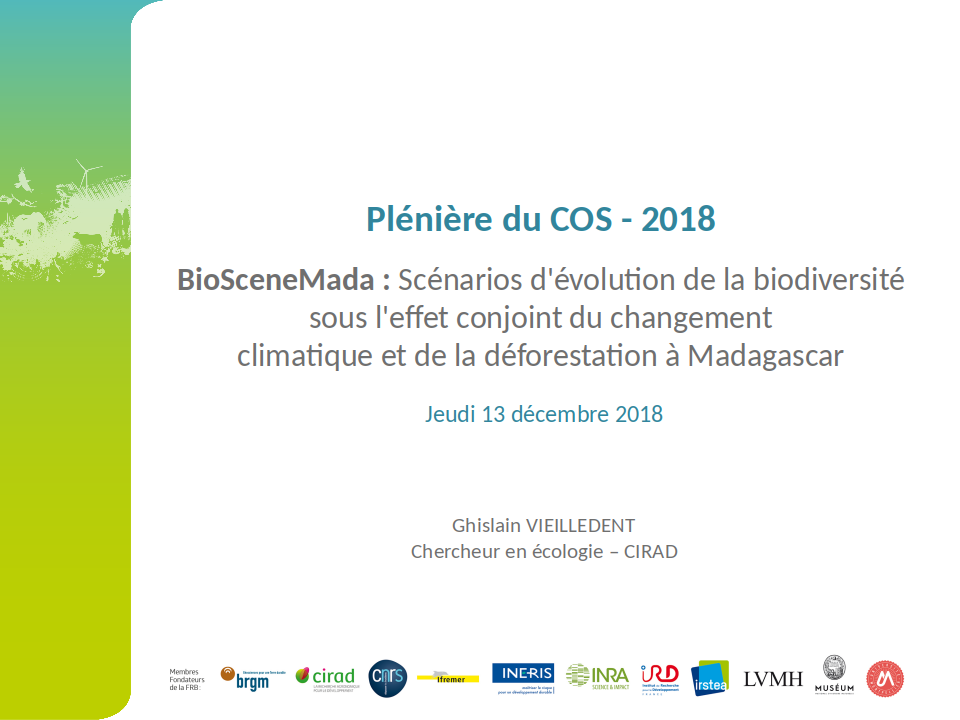
\includegraphics[height=\paperheight,width=\paperwidth]{figs/Masque.png}
%   }
%   \setbeamertemplate{navigation symbols}{}
%   % Remove shadow from block
%   \setbeamertemplate{blocks}[rounded][shadow=false]
%   \begin{frame}[plain]
%   \end{frame}
% }

% Title page
{
  \setbeamertemplate{navigation symbols}{}
  \begin{frame}[plain, noframenumbering]
  \begin{center}
  \small{\textbf{Meeting with Verra -- videoconference, December 2024}}
  \end{center}
  \vspace{-0.5cm}
  \titlepage % Presentation first page
  \vspace{-3cm}
  \begin{center}
    
\includegraphics[width=\textwidth]{figs/Barre_couleur}
    
    \vspace{0.25cm}
    
    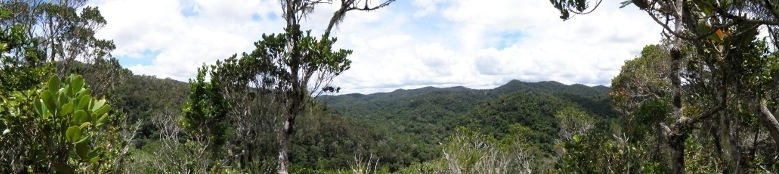
\includegraphics[width=10cm]{figs/Banniere}
    
    \small{Ghislain VIEILLEDENT$^{1}$\hspace{0.25cm}Thomas ARSOUZE$^{1}$\hspace{0.25cm}FAO team$^{2}$}
      
    \vspace{0.25cm}
    
    {\scriptsize
      \begin{tabular}{l}
        $[1]$ \textbf{Cirad} UMR AMAP, $[2]$ \textbf{FAO} Rome
      \end{tabular}
    }
    
    
\includegraphics[width=0.8\textwidth]{figs/partners_logos}
    
  \end{center}
  \end{frame}
}

% %%%%%%%%%%%%%%%%%%%%%%%%%%%%%%%%%%%%%%%%%%%%%%%%%%%%%%%%%%%%%%%%

% \placelogotrue
% \begin{frame}
%   \frametitle{Outline}
%   \begin{columns}[c]
%     \begin{column}{0.5\textwidth}
%       \tableofcontents[sections=1]
%       \vspace{0.5cm}
%       \tableofcontents[sections=2]
%     \end{column}
%     \begin{column}{0.5\textwidth}
%         \tableofcontents[sections=3]
%         \vspace{0.5cm}
%         \tableofcontents[sections=4]
%     \end{column}
%   \end{columns}
% \end{frame}
% \placelogofalse

\section{The deforisk QGIS plugin}
\label{sec:orgf0e5117}

\subsection{Website and documentation}
\label{sec:org625af6b}

\begin{frame}[label={sec:org483833a}]{Website and documentation}
The website includes all the documentation to use the plugin:\\[0pt]

\begin{center}
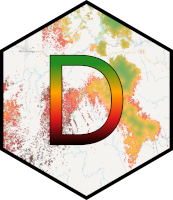
\includegraphics[width=2cm]{figs/logo-deforisk.png}
\end{center}

\centering \url{https://deforisk-qgis-plugin.org}
\end{frame}

\subsection{Aim and specificities}
\label{sec:orgb161bfa}

\begin{frame}[label={sec:orgdbf3a1b}]{Aims and specificities}
\begin{itemize}
\item Provide \textbf{a tool} to create and compare \textbf{deforestation risk maps}.
\item At the \textbf{jurisdictional} level.
\item Following \textbf{Verra's VT0007 v1 principles} (comparison to benchmark map).
\item Open-source and \textbf{Python based}: transparency, reproducibility.
\item Computationally \textbf{efficient} (no need of a large RAM).
\item \textbf{OS independent}: Windows, Linux, MacOS.
\end{itemize}
\end{frame}

\subsection{Alternative models}
\label{sec:orgee36938}

\begin{frame}[label={sec:orgb8af580}]{Alternative models to benchmark}
\begin{itemize}
\item Three statistical models with explanatory variables: iCAR, GLM, Random Forest.
\item One phenomenological model: moving-window model.
\item Map with classes of deforestation risks (up to 65535 classes) and associated deforestation probabilities.
\item Alternative maps can be compared to the benchmark following Verra VT0007-v1.0 2024 methodology.
\item Alternative maps can be used to allocate deforestation to projects within the jurisdiction.
\end{itemize}
\end{frame}

\section{deforisk and VT0007}
\label{sec:orgf90f1de}

\subsection{deforisk alternative maps and VT0007}
\label{sec:org60b74a9}

\begin{frame}[label={sec:orgb0d04e1}]{deforisk alternative maps and VT0007}
\begin{itemize}
\item Alternative maps do not totally match the requisites of Verra VT0007-v1.0 2024.
\item In VT0007:
\begin{itemize}
\item Section 5.4.1 p. 21: Alternative vulnerability maps should have vulnerability scaled from 1 to 30.
\item Section 5.4.2 p. 22: Vulnerability maps should be overlayed with administrative divisions as for the benchmark.
\end{itemize}
\item This is \textbf{not the case} for alternative maps obtained with the deforisk plugin.
\end{itemize}
\end{frame}

\subsection{deforisk validation approach and VT0007}
\label{sec:orge4c1e16}

\begin{frame}[label={sec:org3a52227}]{deforisk validation approach and VT0007}
\begin{itemize}
\item No Theissen polygons are used for validation but a simple regular grid.
\item Additional metrics to the MedAE for validation: R2, RMSE.
\end{itemize}
\end{frame}

\section{Questions and remarks}
\label{sec:orge4f2f71}

\subsection{Regarding VT0007}
\label{sec:org1c55904}

\begin{frame}[label={sec:orgf1451fc}]{Questions regarding VT0007}
\begin{itemize}
\item Is the benchmark model good enough? (cf. hotspots of deforestation within the jurisdictions).
\item Why putting these restrictions on the alternative models. In particular regarding the necessity to overlap with administrative divisions. Several models already incorporate spatial effects to account for regional variability (eg. between administrative divisions).
\item Why using the MedAE and not the R2 and RMSE which are more common?
\item Why using Theissen polygons which implies removing irregular polygons at the edge of the jurisdiction?
\end{itemize}
\end{frame}

\subsection{Regarding deforisk and VT0007}
\label{sec:org4af7ad5}

\begin{frame}[label={sec:orge3c99a4}]{Questions regarding deforisk and VT0007}
\begin{itemize}
\item Have you heard about and tested the deforisk QGIS plugin?
\item What do you think about it, in particular with regards to VT0007?
\end{itemize}
\end{frame}

% %%%%%%%%%%%%%%%%%%%%%%%%%%%%%%%%%%%%%%%%%%%%%%%%%%%%%%%%%%

{
  % Use background image
  \usebackgroundtemplate{%
    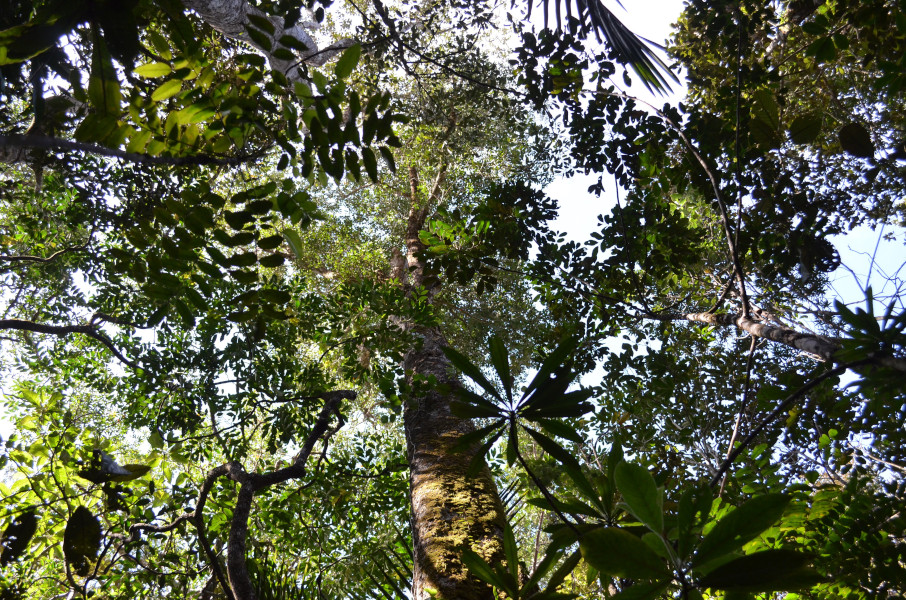
\includegraphics[keepaspectratio=true, height=\paperheight]{figs/Canopy-NC}
  }
  \setbeamertemplate{navigation symbols}{}
  % Remove shadow from block
  \setbeamertemplate{blocks}[rounded][shadow=false]
  \begin{frame}[plain]
  	\vspace*{\stretch{100}} 
    \begin{block}{}
      \begin{center}
        \ldots~Thank you for attention~\ldots \\
        \url{https://deforisk-qgis-plugin.org} \\
        \textbf{> Articles > References > Presentations} \\
        
\includegraphics[width=0.8\textwidth]{figs/partners_logos}
      \end{center}
    \end{block}
  \end{frame}
}
\end{document}
